
\tikzset{every picture/.style={line width=0.75pt}} %set default line width to 0.75pt        
\marginnote{
	\begin{minipage}{5.5cm}
		\begin{figure}[H]\centering
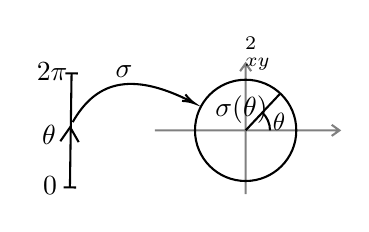
\begin{tikzpicture}[x=0.4pt,y=0.4pt,yscale=-1,xscale=1]
%uncomment if require: \path (0,300); %set diagram left start at 0, and has height of 300

%Shape: Axis 2D [id:dp22600225576346522] 
\draw [color={rgb, 255:red, 128; green, 128; blue, 128 }  ,draw opacity=1 ] (138.75,129.47) -- (305.5,129.47)(220.75,69) -- (220.75,187) (298.5,124.47) -- (305.5,129.47) -- (298.5,134.47) (215.75,76) -- (220.75,69) -- (225.75,76)  ;
%Straight Lines [id:da7351534427888068] 
\draw    (63.5,78) -- (62,181) ;
\draw [shift={(62,181)}, rotate = 270.83] [color={rgb, 255:red, 0; green, 0; blue, 0 }  ][line width=0.75]    (0,5.59) -- (0,-5.59)   ;
\draw [shift={(63.5,78)}, rotate = 270.83] [color={rgb, 255:red, 0; green, 0; blue, 0 }  ][line width=0.75]    (0,5.59) -- (0,-5.59)   ;
\draw   (53.34,139.31) -- (62.21,126.63) -- (69.91,140.06) ;
%Curve Lines [id:da006739188752353686] 
\draw    (64.5,122) .. controls (84.3,87.35) and (114.88,74.26) .. (172.74,104.08) ;
\draw [shift={(174.5,105)}, rotate = 207.72] [color={rgb, 255:red, 0; green, 0; blue, 0 }  ][line width=0.75]    (10.93,-3.29) .. controls (6.95,-1.4) and (3.31,-0.3) .. (0,0) .. controls (3.31,0.3) and (6.95,1.4) .. (10.93,3.29)   ;

%Shape: Circle [id:dp24247899473747292] 
\draw   (175,129.47) .. controls (175,104.2) and (195.48,83.72) .. (220.75,83.72) .. controls (246.02,83.72) and (266.5,104.2) .. (266.5,129.47) .. controls (266.5,154.73) and (246.02,175.22) .. (220.75,175.22) .. controls (195.48,175.22) and (175,154.73) .. (175,129.47) -- cycle ;
%Straight Lines [id:da1420991074145872] 
\draw    (220.75,129.47) -- (251.75,96.47) ;


%Shape: Arc [id:dp4406895489319238] 
\draw  [draw opacity=0] (235.79,113.42) .. controls (240.37,117.7) and (242.74,123.56) .. (242.75,129.47) -- (220.75,129.47) -- cycle ; \draw   (235.79,113.42) .. controls (240.37,117.7) and (242.74,123.56) .. (242.75,129.47) ;

% Text Node
\draw (46,76) node   {$2\pi $};
% Text Node
\draw (44,179) node   {$0$};
% Text Node
\draw (43,134) node   {$\theta $};
% Text Node
\draw (111,76) node   {$\sigma $};
% Text Node
\draw (232,60) node   {$\R^{2}_{xy}$};
% Text Node
\draw (217,111) node   {$\sigma ( \theta )$};
% Text Node
\draw (251,122) node [scale=0.9]  {$\theta $};


\end{tikzpicture}
			\caption{Mapeo de las coordenadas polares.}\label{ch0d6}
		\end{figure}
\end{minipage}}